\ifdefined\COMPILINGFROMMAIN
\else
    %%%%HEADER
\documentclass[twocolumn]{article}
\usepackage[a4paper, margin=1in, columnsep=20pt]{geometry}
\usepackage{amsmath, amssymb, graphicx, hyperref}
\usepackage[most,skins,breakable]{tcolorbox}
\usepackage[symbol]{footmisc}
\usetikzlibrary{calc}
\usepackage{xcolor}
\usepackage{caption}
\usepackage{algorithm}
\usepackage{algpseudocodex}
\usepackage{tikz}
\usepackage{listings}
\usetikzlibrary{arrows.meta, positioning}
\tcbuselibrary{listingsutf8}
\usepackage{microtype}
\usepackage{blindtext}
\usepackage{bookmark}
\usepackage{breqn}
\usepackage[backend=biber,style=numeric]{biblatex} % 
\addbibresource{../references.bib}

% Define style for the listings environment
\lstdefinestyle{mystyle}{
    basicstyle=\ttfamily\small,
    breaklines=true,
    escapeinside={(*@}{@*)}, % Allows math mode within listings
    numbers=left,
    numberstyle=\tiny,
    frame=single,
    keywordstyle=\color{blue}\bfseries,
    commentstyle=\color{green!50!black},
    stringstyle=\color{red}
}


\def\reals{\mathbb{R}}
% Define the custom definition box and command
\newtcolorbox{mydefinition}[2][]{%
    text width=0.95\columnwidth,
    before=\vspace{1mm}, 
    after=\vspace{1mm}, 
    colback=gray!10, % Background color (light gray)
    colframe=black!70,  % Border color
    coltitle=gray!10,  % Title color
    fonttitle=\bfseries, % Title font style
    sharp corners,   % Box style
    left=2pt,
    breakable,
    right=2pt,
    top=2pt,
    bottom=2pt,
    enhanced jigsaw,
    title=Definition: {#1},         % Title passed as the first argument
    colupper=black,  % Ensure proper content handling
    pad at break*=1pc,
    overlay first and middle={
        \coordinate (A1) at ($(interior.south east) + (-10pt,5pt)$);
        \coordinate (C1) at ($(interior.south east) + (-6pt,7.5pt)$);
        \draw[fill=black!50] (A1) -- +(0,5pt) -- (C1) -- cycle;
    }
    }
    
\newcommand{\definition}[2]{%
    \noindent%
    \begin{mydefinition}[#1]%
        .#2%
    \end{mydefinition}%
    \noindent
}

\newtcolorbox{myexample}[2][]{%
    text width=0.95\columnwidth,
    before=\vspace{1mm}, 
    after=\vspace{1mm}, 
    colback=orange!3, % Background color (light gray)
    colframe=black!70,  % Border color
    coltitle=gray!10,  % Title color
    fonttitle=\bfseries, % Title font style
    sharp corners,   % Box style
    left=2pt,
    right=2pt,
    top=2pt,
    bottom=2pt,
    breakable,
    title=Intuition: {#1},         % Title passed as the first argument
    pad at break*=1pc,
    overlay first and middle={
        \coordinate (A1) at ($(interior.south east) + (-10pt,5pt)$);
        \coordinate (C1) at ($(interior.south east) + (-6pt,7.5pt)$);
        \draw[fill=black!50] (A1) -- +(0,5pt) -- (C1) -- cycle;
    }
}

\newcommand{\example}[2]{%
    \noindent%
    \begin{myexample}[#1]%
    .#2%
    \end{myexample}%
    \noindent
}

\newtcolorbox{algobox}[2][]{%
    text width=0.95\columnwidth,
    before=\vspace{1mm}, 
    after=\vspace{1mm}, 
    colback=blue!5, % Background color (light gray)
    colframe=black!70,  % Border color
    coltitle=gray!10,  % Title color
    fonttitle=\bfseries, % Title font style
    sharp corners,   % Box style
    left=2pt,
    right=2pt,
    top=2pt,
    bottom=2pt,
    breakable,
    title=Algorithm: {#1},         % Title passed as the first argument
    pad at break*=1pc,
    overlay first and middle={
        \coordinate (A1) at ($(interior.south east) + (-10pt,5pt)$);
        \coordinate (C1) at ($(interior.south east) + (-6pt,7.5pt)$);
        \draw[fill=black!50] (A1) -- +(0,5pt) -- (C1) -- cycle;
    }
}

\newcommand{\algorithmbox}[2]{%
\noindent%
    \begin{algobox}[#1]%
    .#2%
    \end{algobox}%
    \noindent
}
%%%%HEADER

    \begin{document}
\fi
\noindent
In this second-to-last chapter, we give demonstrations of the Laplacian matrices we have built, solved with the built PN solver from chapter \ref{sec:prior}. We will use the colormap in figure \ref{fig:colorbar} for all figures in this section.
\\
\begin{center}
    
\includegraphics[width=1.0\columnwidth]{../images/colorbar.png}
    \captionof{figure}{Colorbar for the figures in this section, using the perceptually uniform \texttt{viridis} \cite{viridis} colormap. The associated scalar values will generally not be given as they are not important for the interpretation of the figures. Colors will have been renormalized for visualization purposes. However, generally, dark value are negative, light values are positive, and the midpoint is zero.}
    \label{fig:colorbar}
\end{center}
\noindent

\subsection*{Solving the Poisson Problem}
Here are solutions of the Poisson problem on the 2D surface of various shapes - since they are not time-varying, they will not be solved using our PN solver, but can be solved by a linear solver. The Poisson problem is given by:
\begin{align}
    -\Delta u = f
\end{align}
On a mesh with the discrete Laplacian $L$, this reduces to finding the vector $u$ such that $Lu = f$, which is straightforward to solve with numerical linear algebra tools. For this example, we solve the Poisson problem on a model of a twisty section of kelp. The curvature of the kelp is encoded in the Laplacian matrix. Since this two-dimensional surface has a boundary, we must specify boundary conditions: We set both opposing pairs of edges to the same color, some positive and negative value, respectively (Dirichlet boundary conditions). The solution is illustrated in figure \ref{fig:helix}. The topmost figure shows the boundary conditions (the interior is set to zero for this visualization). The middle figure shows the force $f$, which is a positive stretched Gaussian bell on the interior. The bottommost figure shows the computed solution, which satisfies the hot/cold boundary conditions, while the interior satisfies the curvature dictated by $f$.
\newpage
\begin{center}
    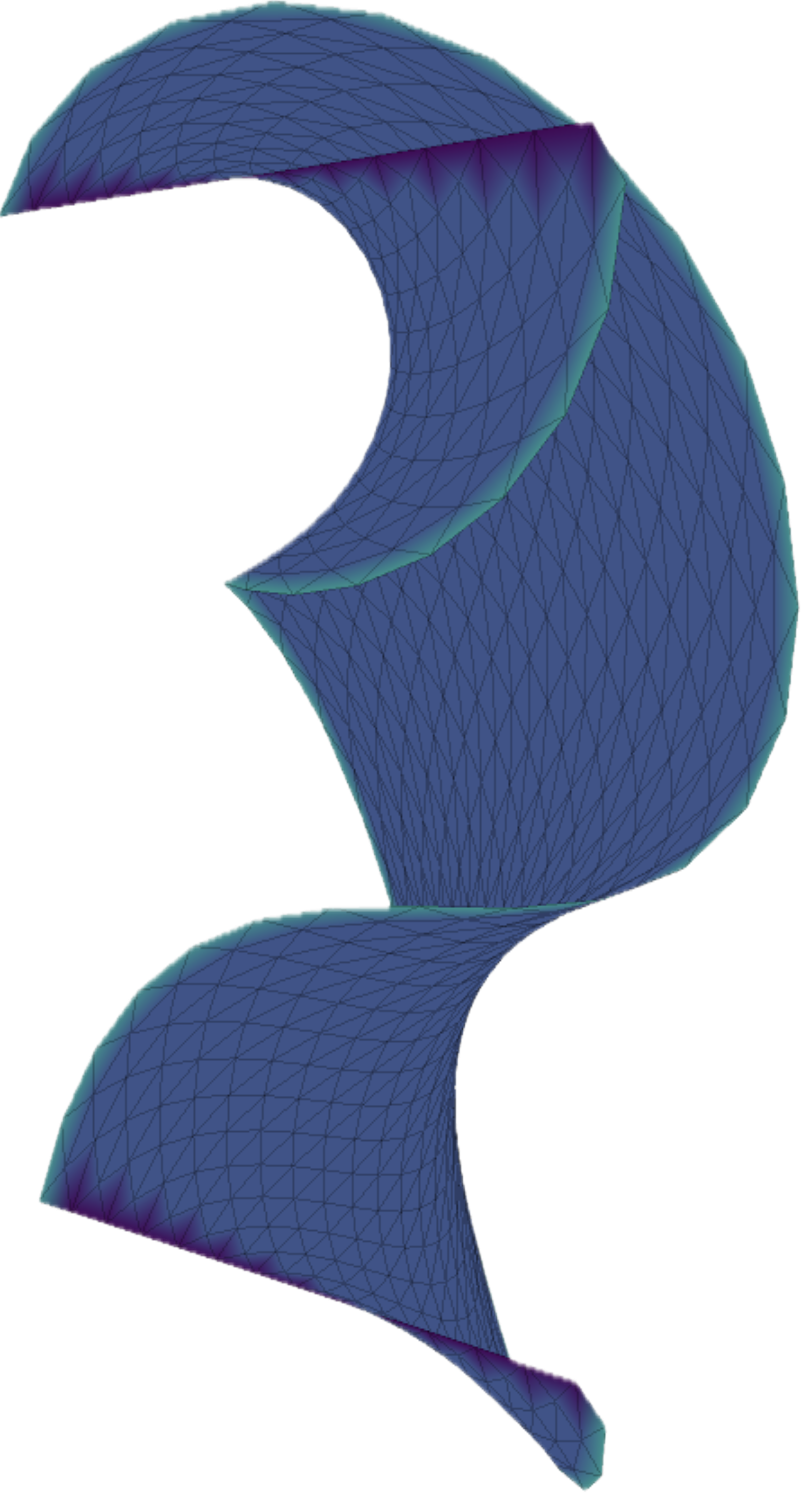
\includegraphics[width=0.95\linewidth]{../images/helix_BC.png}
    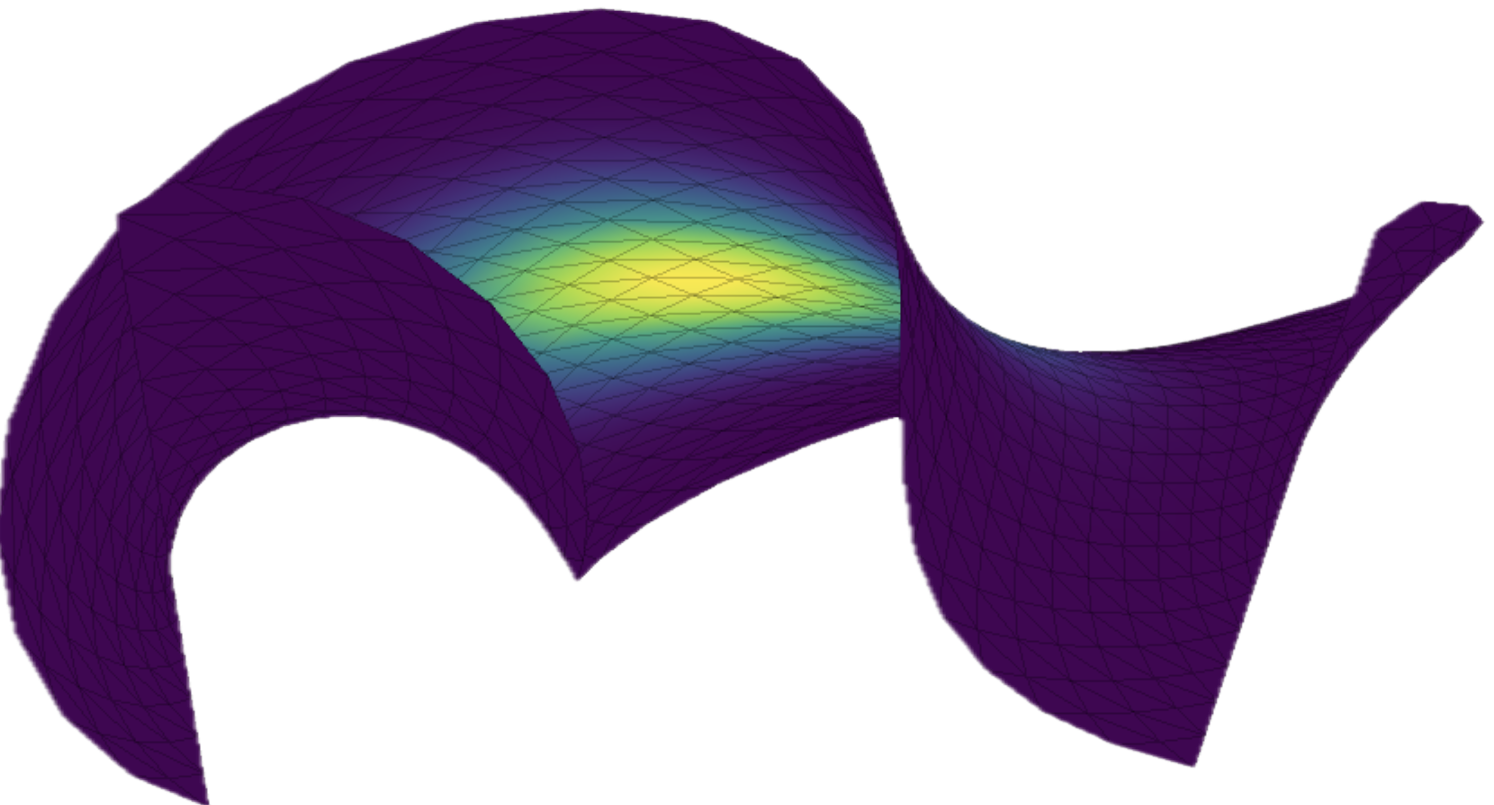
\includegraphics[width=0.95\linewidth]{../images/helix_force.png}    
    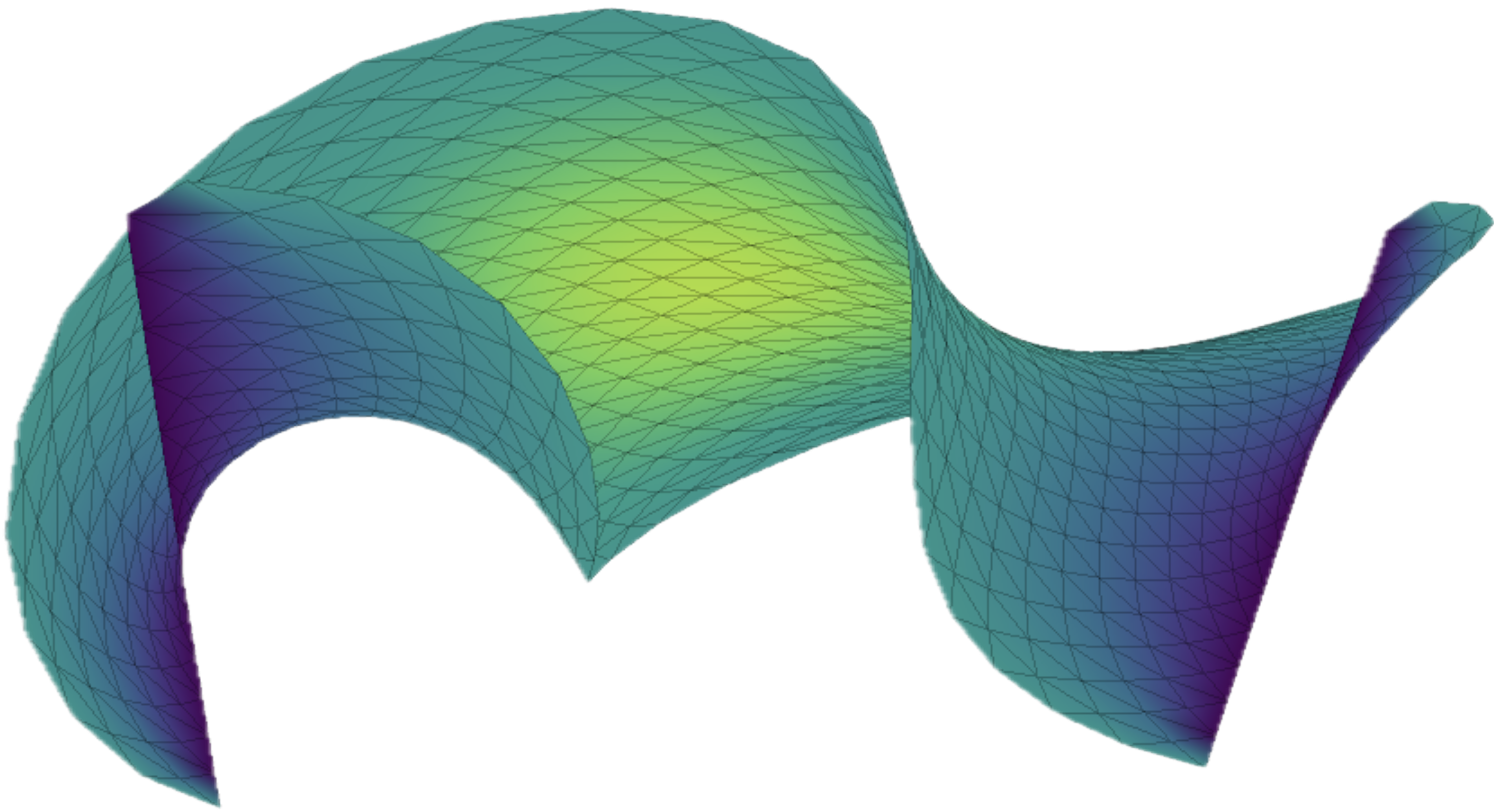
\includegraphics[width=0.95\linewidth]{../images/helix_solution.png}
    \captionof{figure}{}
    \label{fig:helix}
\end{center}


\subsection*{Solving the Heat Equation}
We solve the heat equation on the sphere, using the twice-integrated Wiener process, see figure \ref{fig:heat_solution} for the mean of the process at selected timesteps. In figure \ref{fig:heat_uncertainty} we show the marginal uncertainties of the solution. We interpret the nonuniformity of the figure in the following way: The sphere mesh used has twelve\footnote{This mesh is created by using loop subdivision on the 12-tipped icosahedron with the \texttt{icosphere} Python package, which is a coarse approximation to the sphere geometry.} patches of vertices with incidence number 5 - in these, the solution is more certain than in the remaining ones. The Laplacian matrix will have five nonzero entries in the corresponding rows instead of six, and thus the solution here is less sensitive to the values of the neighbors. Additionally, the neighboring five vertices are spatially closer (the edge lengths are shorter), which introduces higher correlation between them, reducing overall uncertainty.

\begin{center}
    \begin{minipage}[b]{0.5\columnwidth}
        \centering
        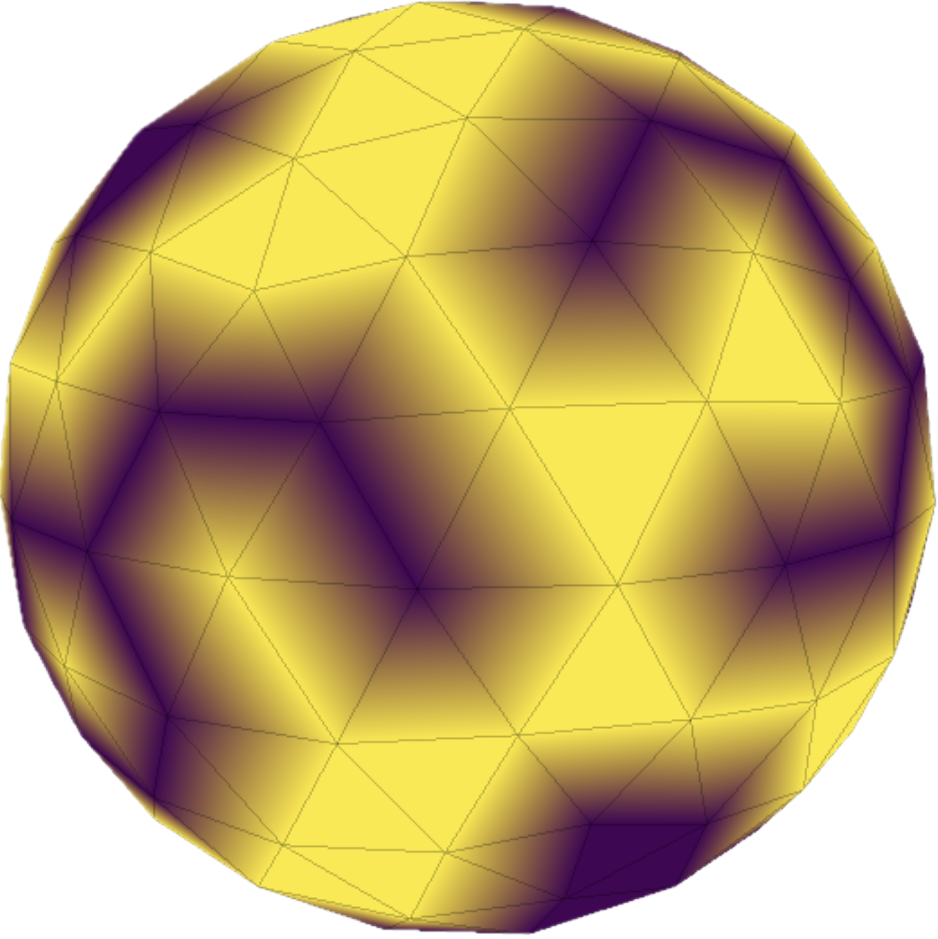
\includegraphics[width=0.95\linewidth]{../images/sphere_entropic.png}
    \end{minipage}%
    % \hspace{5mm} 
    \begin{minipage}[b]{0.5\columnwidth}
        \centering
        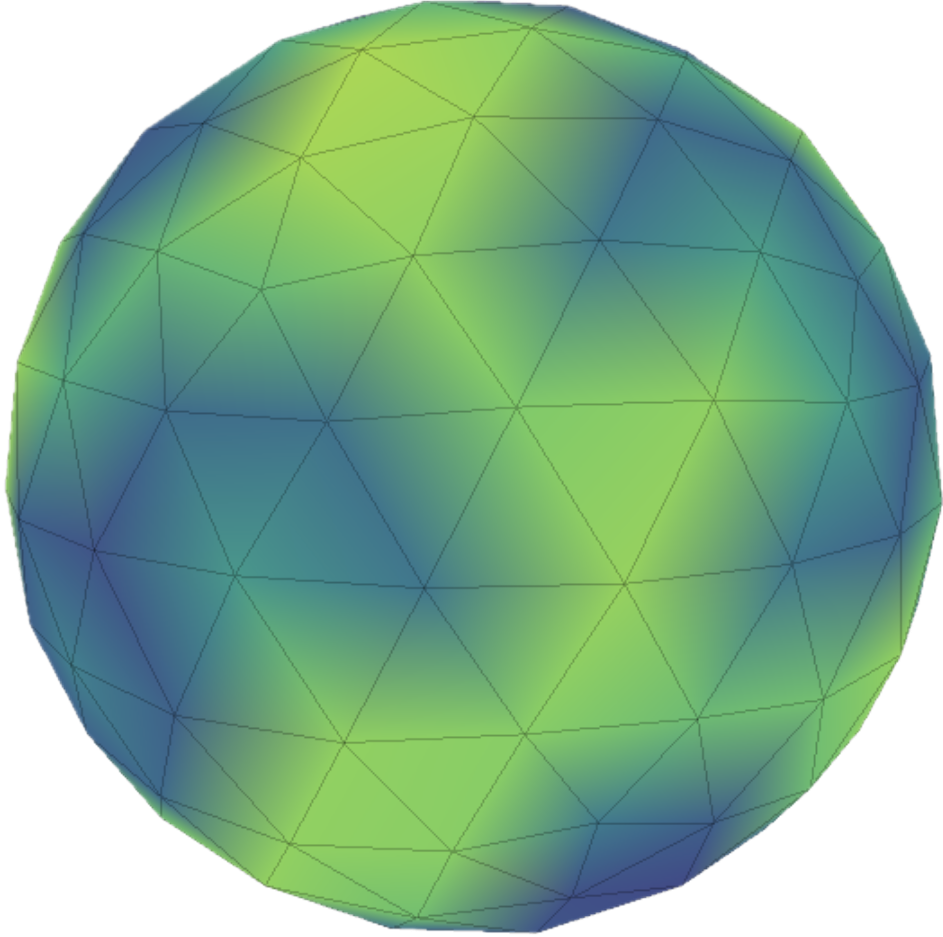
\includegraphics[width=0.95\linewidth]{../images/sphere_smoothed.png}
    \end{minipage}
    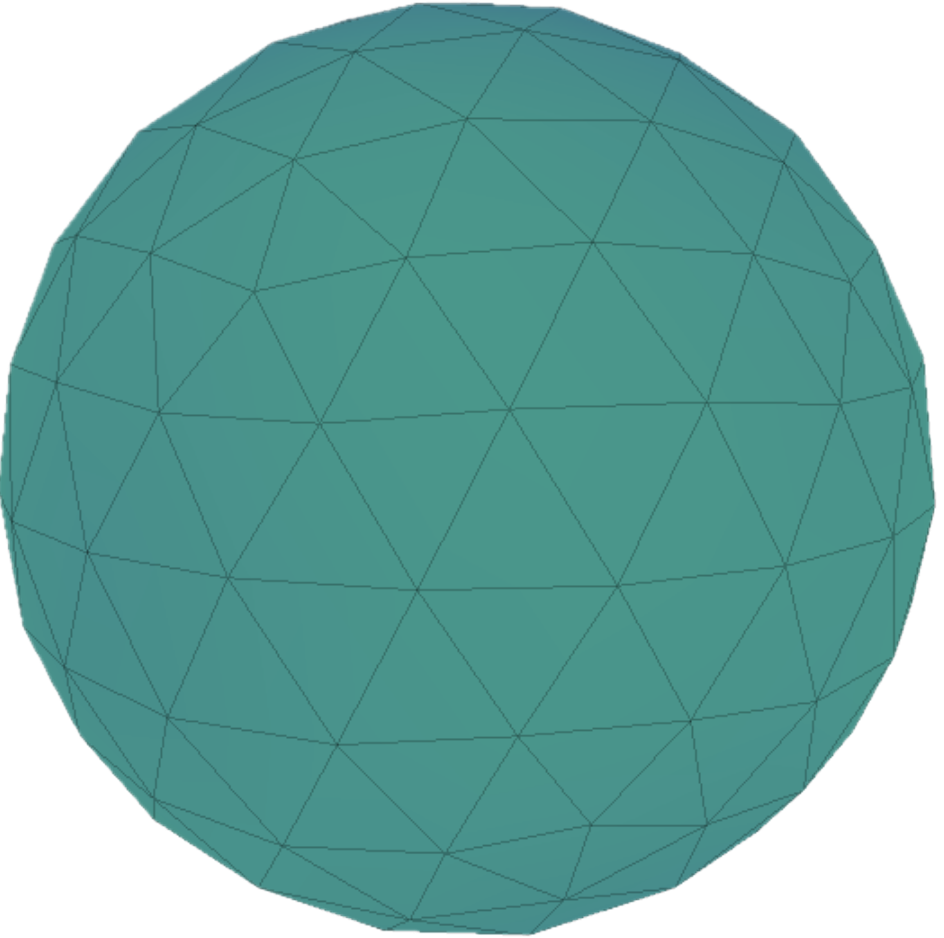
\includegraphics[width=0.475\columnwidth]{../images/sphere_cooled.png}\vspace*{3mm}
    \captionof{figure}{The heat equation solved on the sphere. Upper left image is the initial temperature distribution, where each vertex has been assigned to $\{-1, 1\}$ uniformly at random. Upper right and lower image are spaced equally apart in time, illustrating the heat diffusion. Yellows are positive temperatures, blues are negative temperatures.}
    \label{fig:heat_solution}
\end{center}

\begin{center}
    \vspace{10mm}
    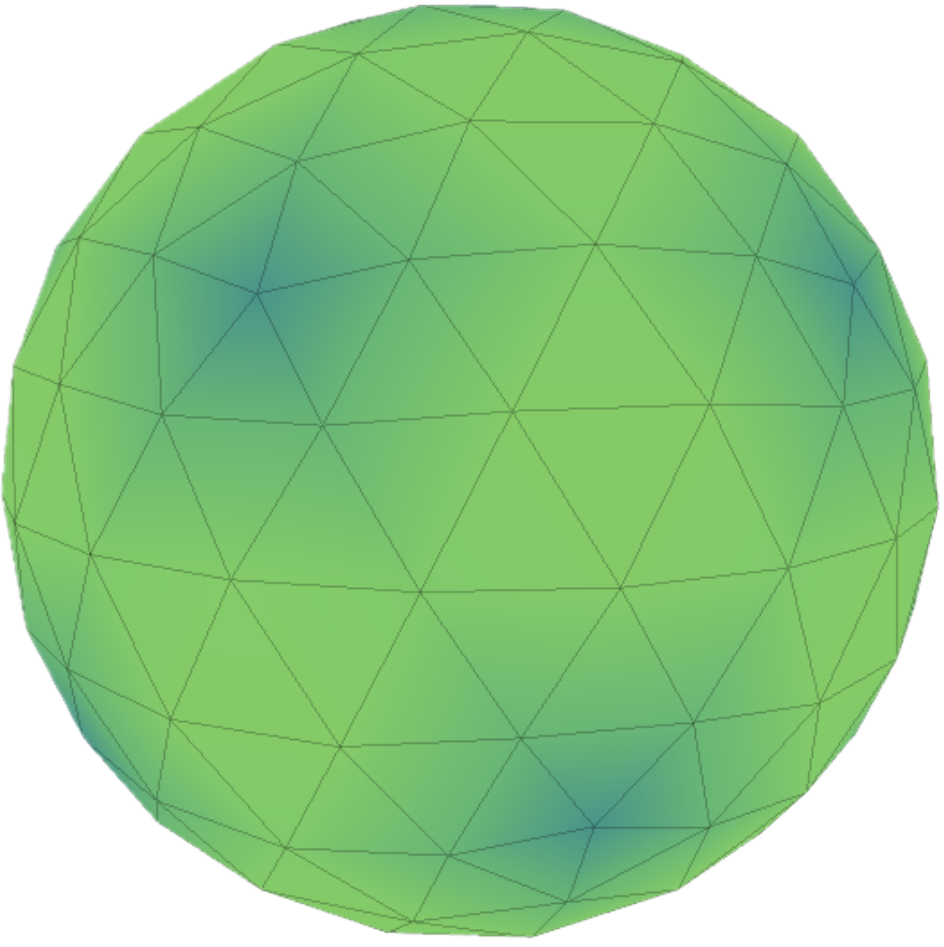
\includegraphics[width=0.7\columnwidth]{../images/sphere_uncertainty.png}\vspace*{3mm}
    \captionof{figure}{The marginal standard deviations of the solution at the second step in figure \ref{fig:heat_solution}. Darker colors mean lower uncertainty. The uncertainty is miniscule and has been scaled up for illustration.}
    \label{fig:heat_uncertainty}
\end{center}

\example{The Laplacian captures the length-scale}{   
The speed of diffusion is linked to the Laplacian matrix $L$ and depends on the scale of the geometry. We visualize this dependence on the Utah teapot \cite{utah}, scaled so the body of the teapot is approximately a unit sphere. Figure \ref{fig:teapot_heat_solution} shows the heat equation initial step and a short time later. The teapot has non-uniform dual face areas, especially around the rim at the lid. That the diffusion process is not scale-invariant is illustrated by the fact that the temperature here will smooth out much quicker than in the remaining, bigger patches.
    \begin{center}
        \centering
        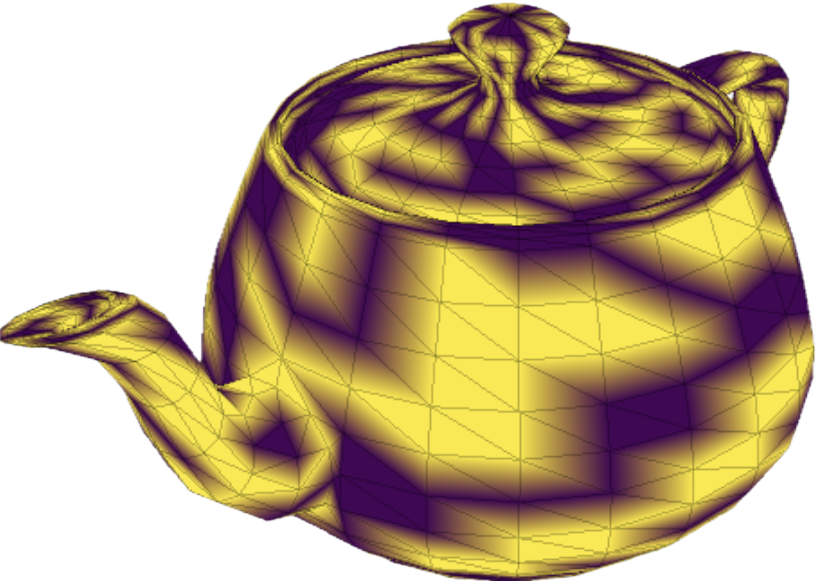
\includegraphics[width=0.9\columnwidth]{../images/teapot_entropic.png}\vspace*{3mm}
        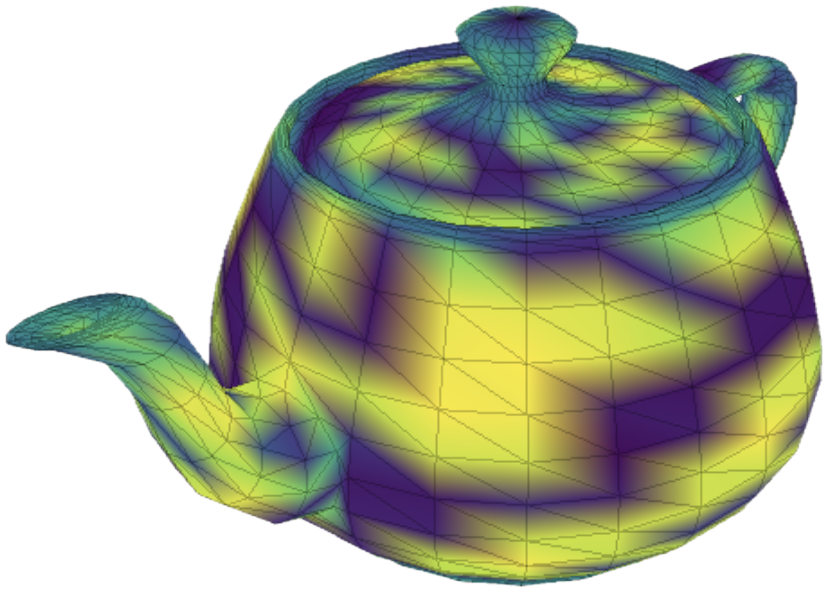
\includegraphics[width=0.9\columnwidth]{../images/teapot_smoothed.png}\vspace*{3mm}
        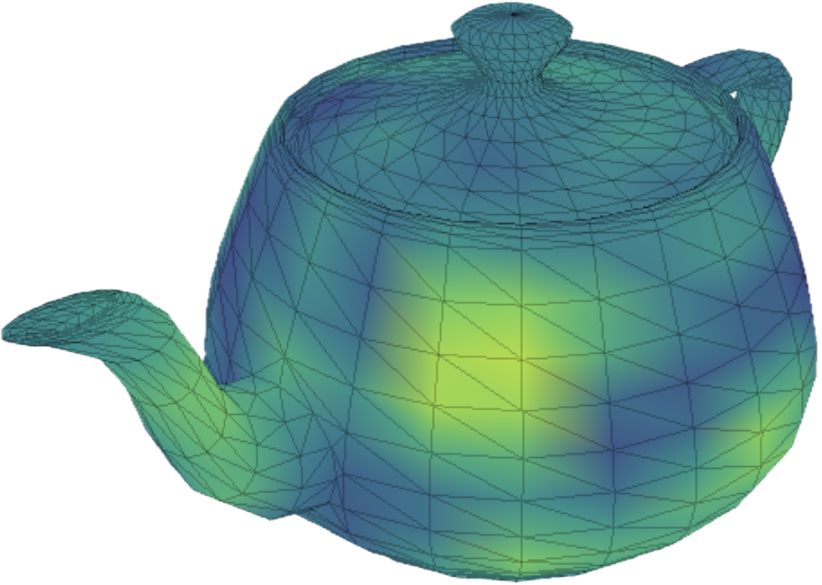
\includegraphics[width=0.9\columnwidth]{../images/teapot_cooled.png}\vspace*{3mm}
        \captionof{figure}{The heat equation being solved on the Utah Teapot. Top: The initial conditions are akin to the ones in fig. \ref{fig:heat_solution} and shown in the topmost figure. Middle: Heat diffusion after a short time. Bottom: Heat diffusion after a longer time.}
        \label{fig:teapot_heat_solution}
    \end{center}
}

\subsection*{Solving the Wave Equation On an Intrinsically Triangulated Surface}
Using our algorithm from chapter \ref{sec:intrinsic_triangulation}, we use triangulate the bell-curve geometry, compute the Laplacian, and solve the wave equation on it. To motivate the expected behaviour, one can think of a wave as simply a shockwave traveling at constant speed from a source, which we visualize an approximation of in figure \ref{fig:dijkstra}. There are multiple ways to compute the location of the front of the shockwave, such as the ones proposed and compared in \cite{vector_dijkstra} and \cite{heat_method}. For the sake of ease of implementation, we use the simplest one, Dijkstra's single-source-all-paths algorithm. The figure shows level-sets of the distance function to the source (on the left, at coordinates $(-0.5, 0.0)$). This figure suggests that one should observe the wave traveling around the bump faster than across it, which is reasonable, given the detour the wave would take to travel across the bump.
This simplification ignores the reflections and interference that might occur due to our Dirichelet BCs (which are fixed at a wave-height of zero).
\\
The four stacked planes in figure \ref{fig:bell_wave}, show the solution of the wave equation on the intrinsic bell-curve mesh.
\label{fig:bell_wave}
\newpage
\begin{center}
    \centering
    \hspace*{-6mm}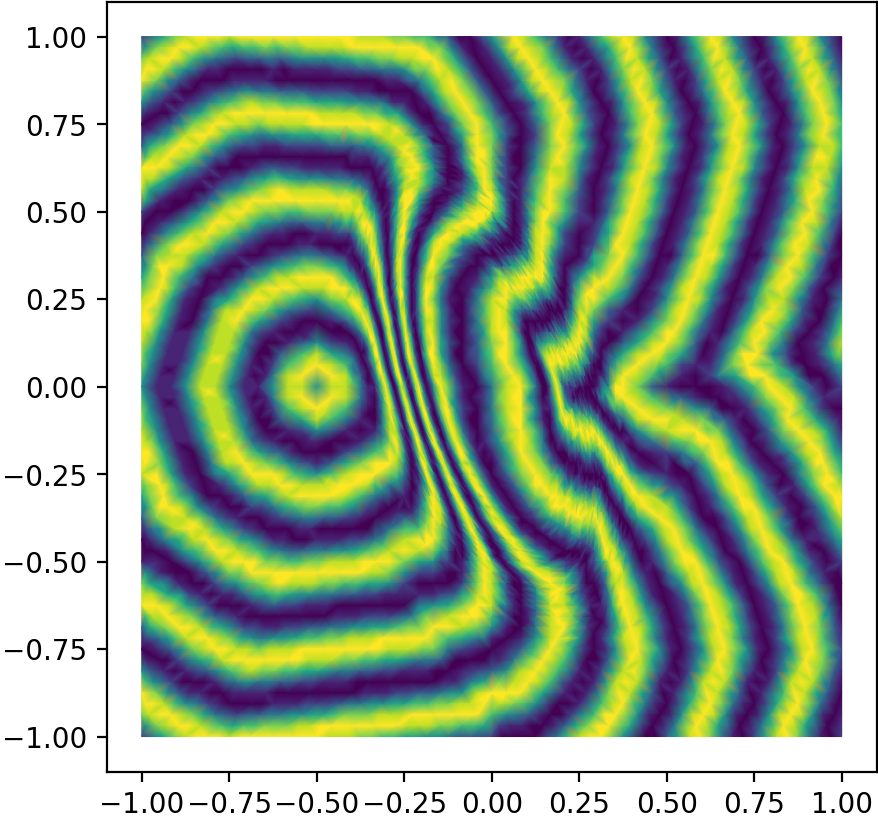
\includegraphics[width=0.9\columnwidth]{../images/bell_wave_distances.png}
    \captionof{figure}{Level sets of the distance function from a source at coordinates $(-0.5, 0.0)$ on the intrinsic triangulation of the Gaussian bump mesh. The wave equation is solved on this mesh in the following figure.}
    \label{fig:dijkstra}
    \vspace*{10mm}
    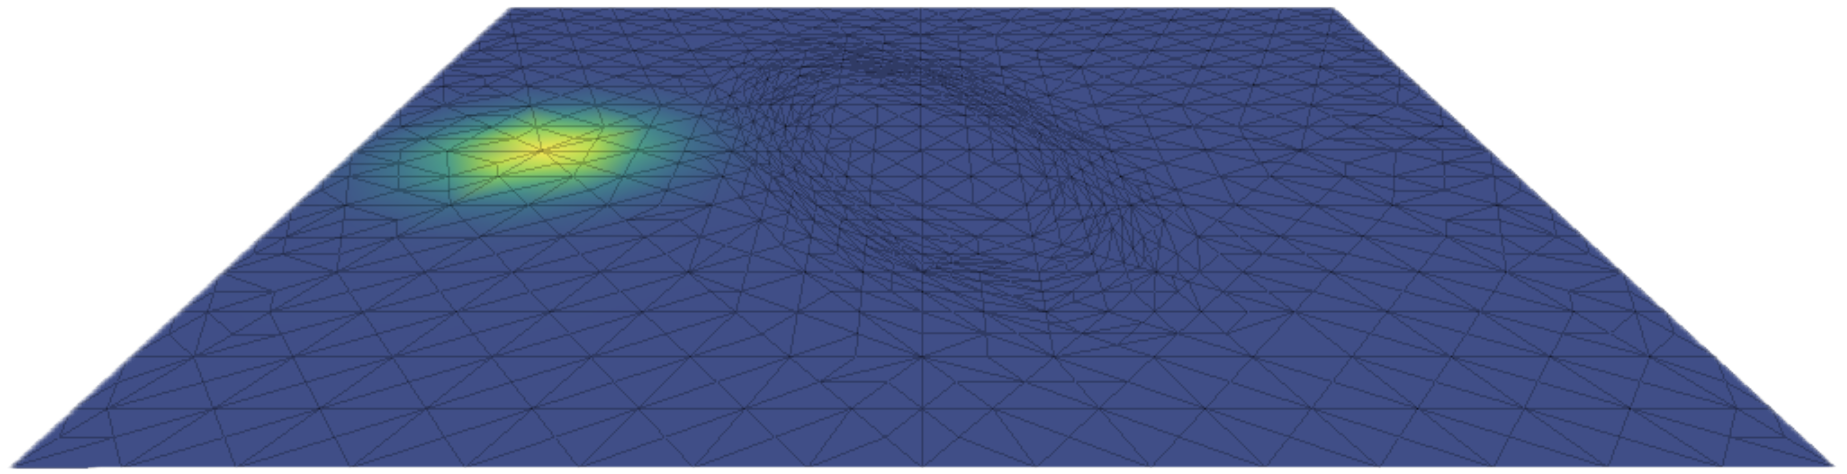
\includegraphics[width=\columnwidth]{../images/bell_wave_0.png}\vspace*{3mm}
    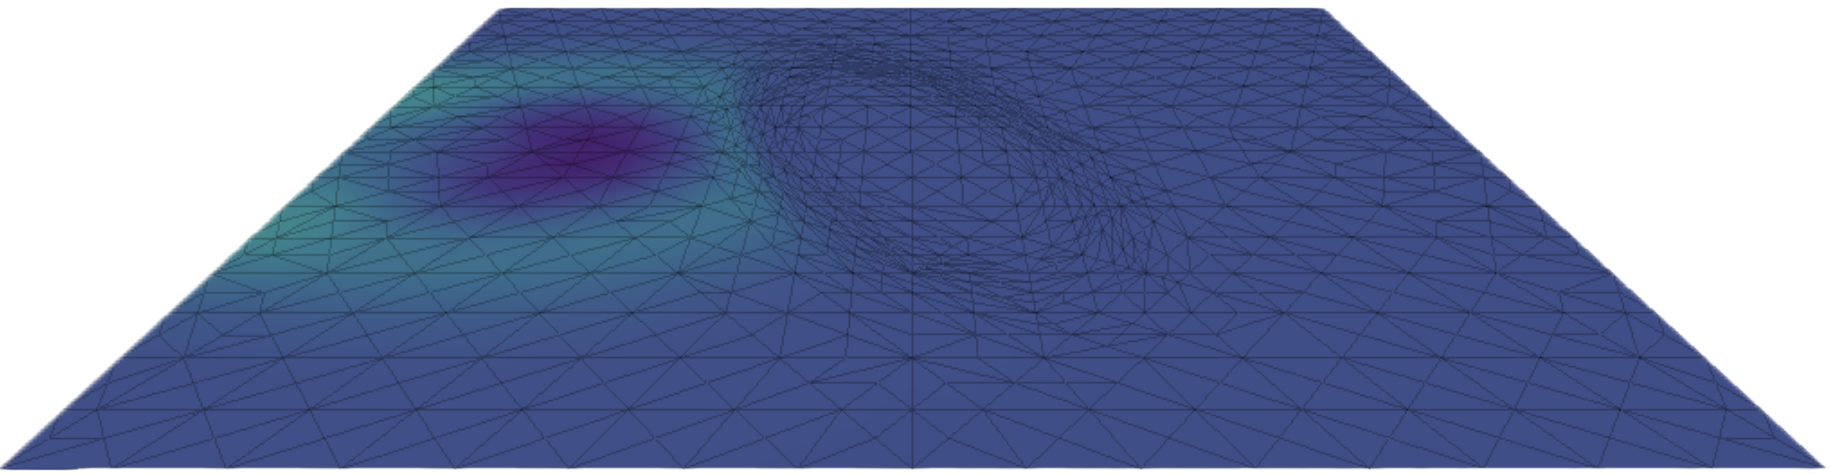
\includegraphics[width=\columnwidth]{../images/bell_wave_1.png}\vspace*{3mm}
    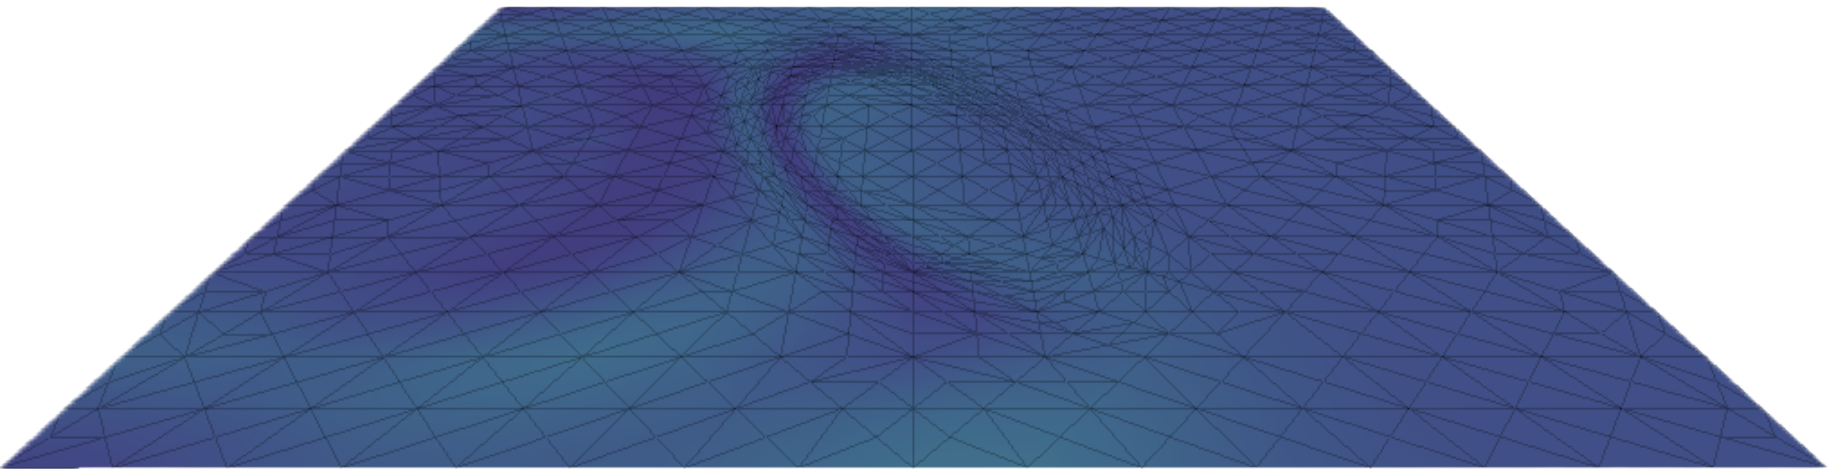
\includegraphics[width=\columnwidth]{../images/bell_wave_2.png}\vspace*{3mm}
    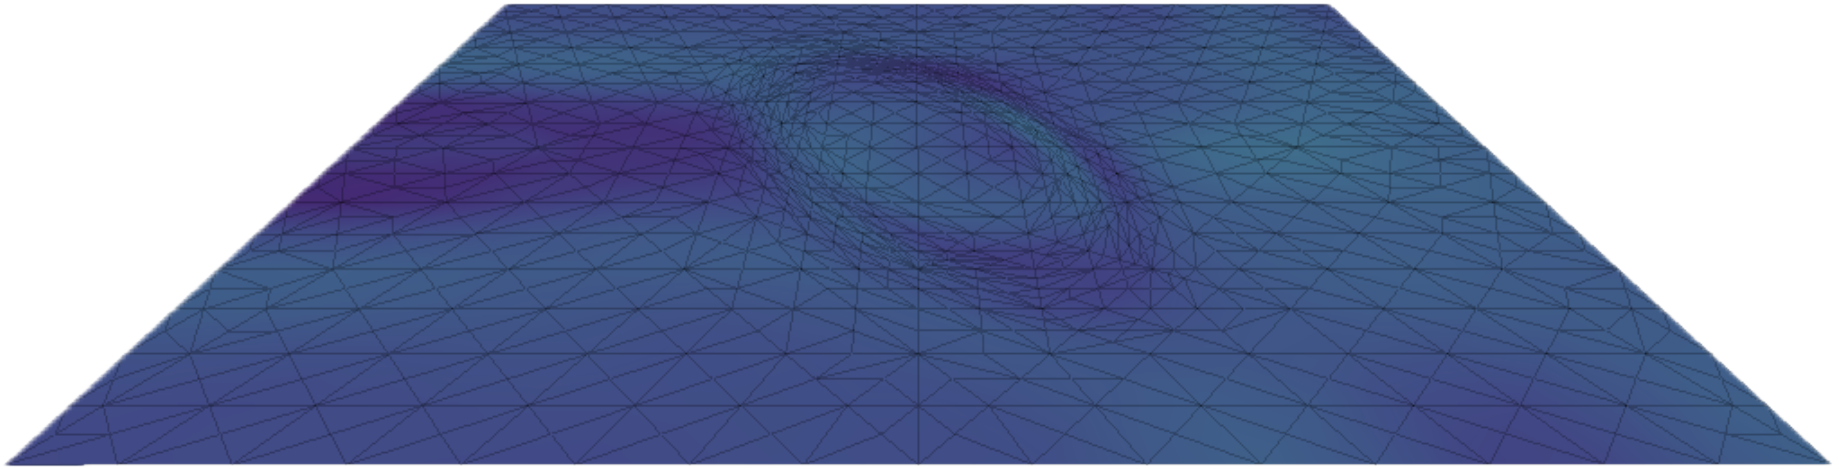
\includegraphics[width=\columnwidth]{../images/bell_wave_3.png}\vspace*{3mm}
    \captionof{figure}{From top to bottom, four consecutive equally spaced instants of the wave equation on the intrinsic triangulation of the Gaussian bump mesh. The initial condition is given in the topmost picture. In the third picture from the top, there are clear similarities with the shapes shown in \ref{fig:dijkstra} when comparing the shape of the wave around the bump. We emphasize that the mesh is completely intrinsic and "flat" - there is no extrusion of the bump on this mesh.}
    \label{fig:bell_wave}
\end{center}

\section{Experiments with Physically Informed Priors}
In this final short chapter, we will demonstrate the efficiency of the probabilistic solver when using physically informed priors. As problems to solve, we choose a nonlinear version of the heat (\ref{eq:nonlinear_heat}) and wave (\ref{eq:nonlinear_wave}) equation, with varying degrees of nonlinearity. 
\begin{align}
    \frac{\partial}{\partial t}u = -\Delta u - \alpha u^2\label{eq:nonlinear_heat}
\end{align}
\begin{align}
    \frac{\partial^2}{\partial t^2}u = -\Delta u - \alpha\tan u\label{eq:nonlinear_wave}
\end{align}
The hypothesis is that, for small nonlinearities, a prior that encodes the linear heat/wave dynamics will outperform the integrated Wiener process. 

\subsection*{Encoding the Linear part of a PDE into a Prior}
This idea is adapted from \cite{exponential_probabilistic} in which the authors show that using integrated Ornstein-Uhlenbeck processes (chapter \ref{sec:prior}) give an inductive bias when solving ODEs with partially linear dynamics. Using such a prior leads to faster convergence than the usual integrated Wiener process, because it exactly solves the linear part of the ODE.
We show that the same idea can be applied to PDEs and give appropriate prior process, but will start by explaining the principle.
\\
\example{Mean of Prior solves Linear ODE exactly}{
We can take any linear ODE and make a series of transformations to the ODE that preserve the modeled system, but will explicitly model more derivatives in the state-space.
\\
We will show the procedure with the damped harmonic oscillator
\begin{align}
    \frac{d}{dt}\vec{u}_0 &= \vec{u}_1 \label{eq:physics_prior_0}
    \\\frac{d}{dt}\vec{u}_1 &= -a\vec{u}_{0} - b\vec{u}_{1}\label{eq:physics_prior_1}
\end{align}
for some fixed choice of $a$, $b$.
\\
Assume we are given initial condition $\vec{u}_0(0)=s_0(0)$, $\vec{u}_1(0) = s_1$. We can feed the initial known values into eq. \ref{eq:physics_prior_1} to get $s_2 = \vec{u}_2(0) = -a\vec{u}_{0}(0) - b\vec{u}_{1}(0)$.
We now impose regularity on $\vec{u}_2$ by taking the derivative w.r.t. time on all terms in the equations \ref{eq:physics_prior_0} and \ref{eq:physics_prior_1}:
\begin{align*}
    \frac{d^2}{dt^2}\vec{u}_0 &=  \frac{d}{dt}\vec{u}_1 \nonumber
    \\
    \frac{d^2}{dt^2}\vec{u}_1 &=  \frac{d}{dt} \left(-a\vec{u}_{0} - b\vec{u}_{1}\right)
    \\
    &=  -a\frac{d}{dt}\vec{u}_{0} - b\frac{d}{dt}\vec{u}_{1}
\end{align*}
By the derivative/integral relationship in the state-space representation, this simplifies to
\begin{align}
    \frac{d}{dt}\vec{u}_0 &= \vec{u}_1
    \\
    \frac{d}{dt}\vec{u}_1 &= \vec{u}_2 \nonumber
    \\
    \frac{d}{dt}\vec{u}_2 &= -a\vec{u}_{1} - b\vec{u}_{2}
\end{align}
We have increased the state-space to encompass another derivative. Since we previously determined $\vec{u}_2(0) = s_2$, we have all the required information to solve this ODE.
\\ The steps in this transformation can be repeated indefinitely; one needs to compute the induced initial value of the derivative from the set of equations and then augment the state-space.
We start off with system matrix $F^\prime$, and after $q-1$ repetitions we end up with a system matrix $F\in\reals^{q+1\times q+1}$ 
$$F^\prime\!\! =\! \begin{bmatrix}
0 & 1 \\  \!-a & \!-b
\end{bmatrix} \to F =\! \begin{bmatrix}
0 & 1 & 0 & \!\!\dots\!\! & 0 & 0 & 0 \\
0 & 0 & 1 & \!\!\dots\!\! & 0 & 0 & 0 \\
0 & 0 & 0 & \!\!\dots\!\! & 0 & 0 & 0 \\
\vdots & \!\!\ddots\!\! & \!\!\ddots\!\! & \!\!\ddots\!\! & \!\!\ddots\!\! & \!\!\ddots\!\! & \vdots \\
0 & 0 & 0 & \!\!\dots\!\! & 0 & 1 & 0 \\
0 & 0 & 0 & \!\!\dots\!\! & 0 & 0 & 1 \\
0 & 0 & 0 & \!\!\dots\!\! & 0 & \!\!-a & \!\!\!\!-b \\
\end{bmatrix}$$
The original system matrix $F'$ is nested inside $F$. \\
We conclude by transforming this into a LTI SDE by adding zero mean Brownian motion increments into the highest derivative. When integrated, it will still have zero mean and therefore will not affect the mean of the process. This is similar in spirit to the spring example in chapter \ref{sec:prior}, and yields the following LTI SDE which can directly be applied as a prior.
\begin{align*}
    \frac{d}{dt}\vec{U}_i &= \vec{U}_{i+1} \hspace{10mm} i \in \{0, \dots, q\!-\!1\}
    \\d\;\vec{U}_q &= -b\vec{U}_{q-2}dt - a\vec{U}_{q-1}dt + \sigma dW(t)
\end{align*}
}
\noindent
The previous example was for scalar-valued ODEs, but the same principle can be applied to the state-space representation of vector-valued ODEs like the ones given at the end of chapter \ref{sec:prior}, which can be obtained after applying the Method of Lines to a PDE. The same principle is then simply applied component-wise. For a dimension $n$ vector-valued linear ODE $$\frac{d^2}{dt^2}u = Au + B\frac{d}{dt}u$$ with state-space system matrix $F^\prime$, the corresponding q-times integrated prior will be constructed as
$$F^\prime\!\! =\! \begin{bmatrix}
    \mathbf{0} & \textbf{I}_n \\ \!A & \!B
    \end{bmatrix} \to F = \begin{bmatrix}
\mathbf{0} & \textbf{I}_n & \mathbf{0} & \!\!\!\dots\!\! & \mathbf{0} & \mathbf{0} & \!\!\mathbf{0} \\
\mathbf{0} & \mathbf{0} & \textbf{I}_n & \!\!\!\dots\!\! & \mathbf{0} & \mathbf{0} & \!\!\mathbf{0} \\
\mathbf{0} & \mathbf{0} & \mathbf{0} & \!\!\!\dots\!\! & \mathbf{0} & \mathbf{0} & \!\!\mathbf{0} \\
\vdots & \!\!\ddots\!\! & \!\!\ddots\!\! & \!\!\ddots\!\! & \!\!\ddots\!\! & \!\!\ddots\!\! & \!\!\vdots \\
\mathbf{0} & \mathbf{0} & \mathbf{0} & \!\!\!\dots\!\! & \mathbf{0} & \textbf{I}_n & \!\!\mathbf{0} \\
\mathbf{0} & \mathbf{0} & \mathbf{0} & \!\!\!\dots\!\! & \mathbf{0} & \mathbf{0} & \textbf{I}_n \\
\mathbf{0} & \mathbf{0} & \mathbf{0} & \!\!\!\dots\!\! & \mathbf{0} & \!\!A & \!\!\!\!B \\
\end{bmatrix}$$
We then build the LTI SDE with the diffusion matrix $LL^\top = E_qE_q^\top$, which ensures that the noise is only fed into the highest derivative. \\
This process of repeated integration yields a LTI SDE with $q$ continuous derivatives whose mean coincides with the solution of the original ODE. We visualize this property for the scalar wave equation and then give the PDE-wave equation counterpart.
\definition{Wave Process}{
    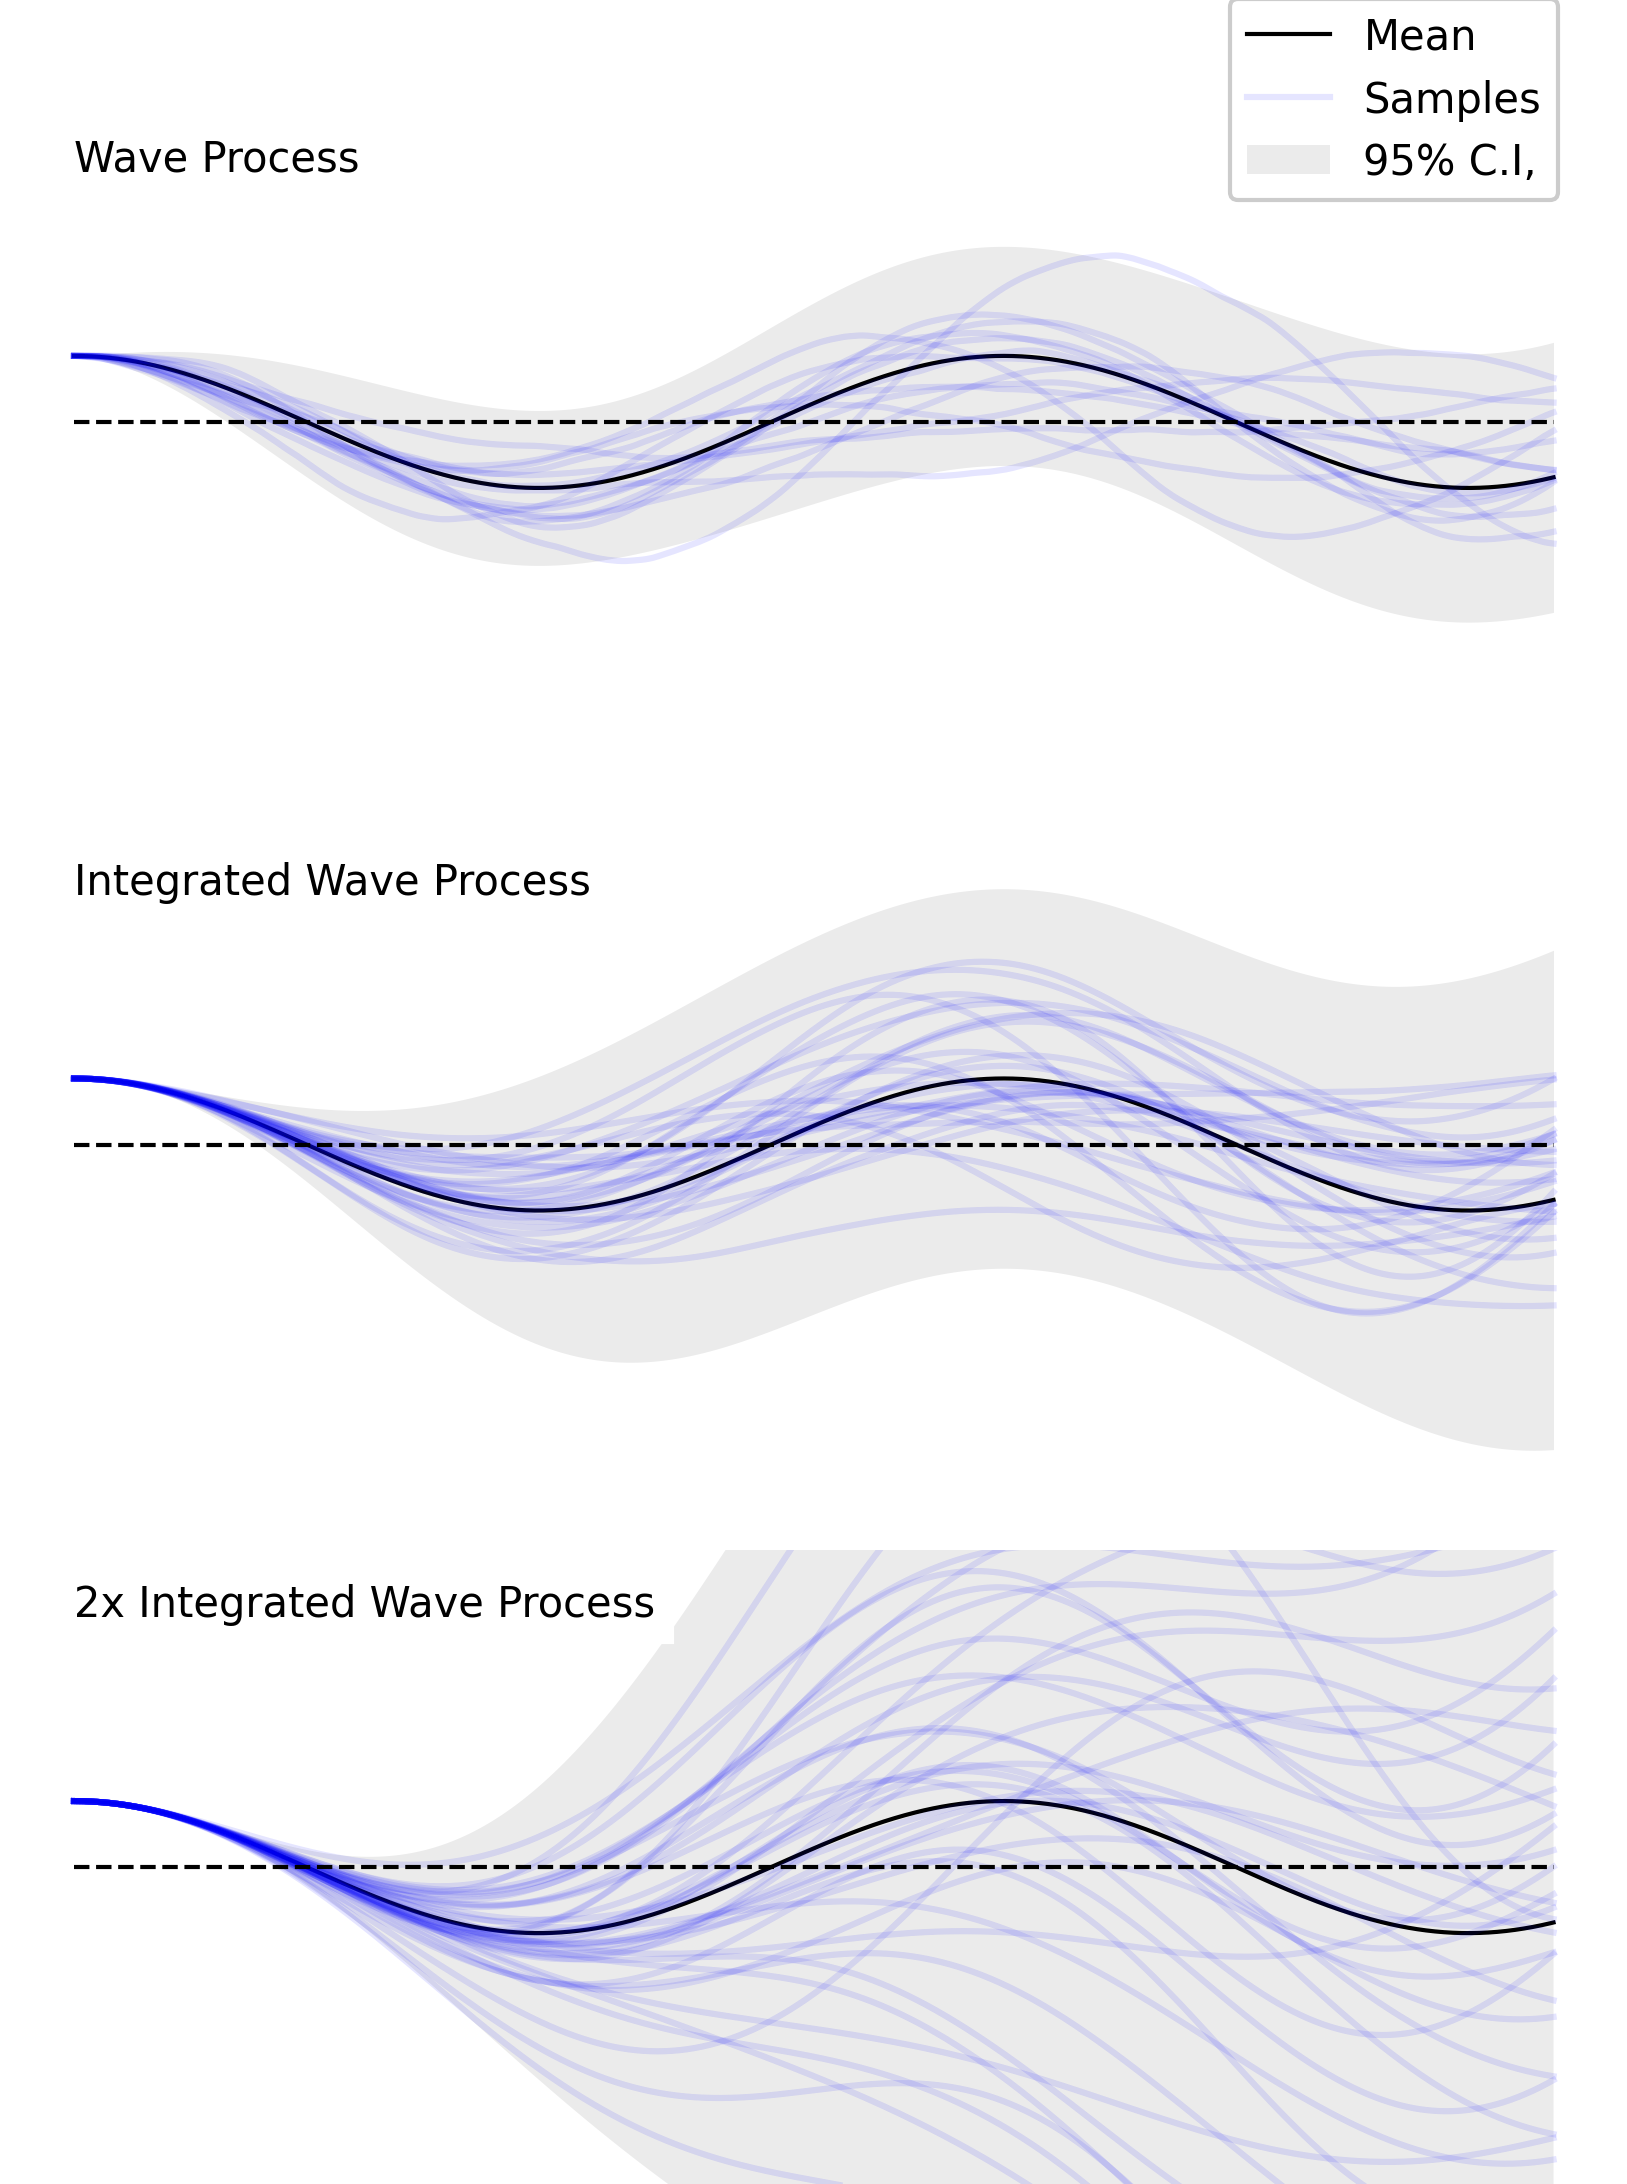
\includegraphics[width=\columnwidth]{../images/wave_process.png}
    \captionof{figure}{Iterated integrations of the Wave Process.}
    \label{fig:wave_process}
    The mean of the scalar Wave process solves the scalar wave equation $\frac{d^2}{dt^2}u = -au$ exactly. The simplest scalar Wave process has system matrix $F$
    $$F = \begin{bmatrix} 0 & 1 \\ -a & \!0 \end{bmatrix} \hspace*{10mm} L = \begin{bmatrix} 0 \\ 1 \end{bmatrix}$$ 
    (shown at the top), while the once-integrated (middle) Wave process has system matrix $F$
    $$F = \begin{bmatrix} 0 & 1 & 0 \\ 0 & 0 & 1 \\ 0 & -a & \!0 \end{bmatrix} \hspace*{10mm} L = \begin{bmatrix} 0 \\ 0 \\ 1 \end{bmatrix}$$
    We initialize the process with the initial conditions calculated from the ODE ($s_0, s_1, \dots$), and the mean will then satisfy the ODE exactly (fig. \ref{fig:wave_process}). The exact solution for $a=1$ is $\cos(t)$.
    \\
    \\
    The corresponding process for the wave equation $\frac{d^2}{dt^2}u = -\Delta u$ can be built by discretizing the Laplacian matrix $L$ and using the Wave process as the prior, 
    $$F = \begin{bmatrix}
    \mathbf{0} &  \textbf{I}_n  \\ \!-L & \! \mathbf{0}
    \end{bmatrix} \hspace*{5mm} LL^\top = E_1E_1^\top = \begin{bmatrix}
    \mathbf{0} & \mathbf{0} \\ \mathbf{0} & \textbf{I}_n \end{bmatrix}$$
    We will denote this SDE as the Wave Process.
}
\example{Wave Process in Action}{
\begin{center}
    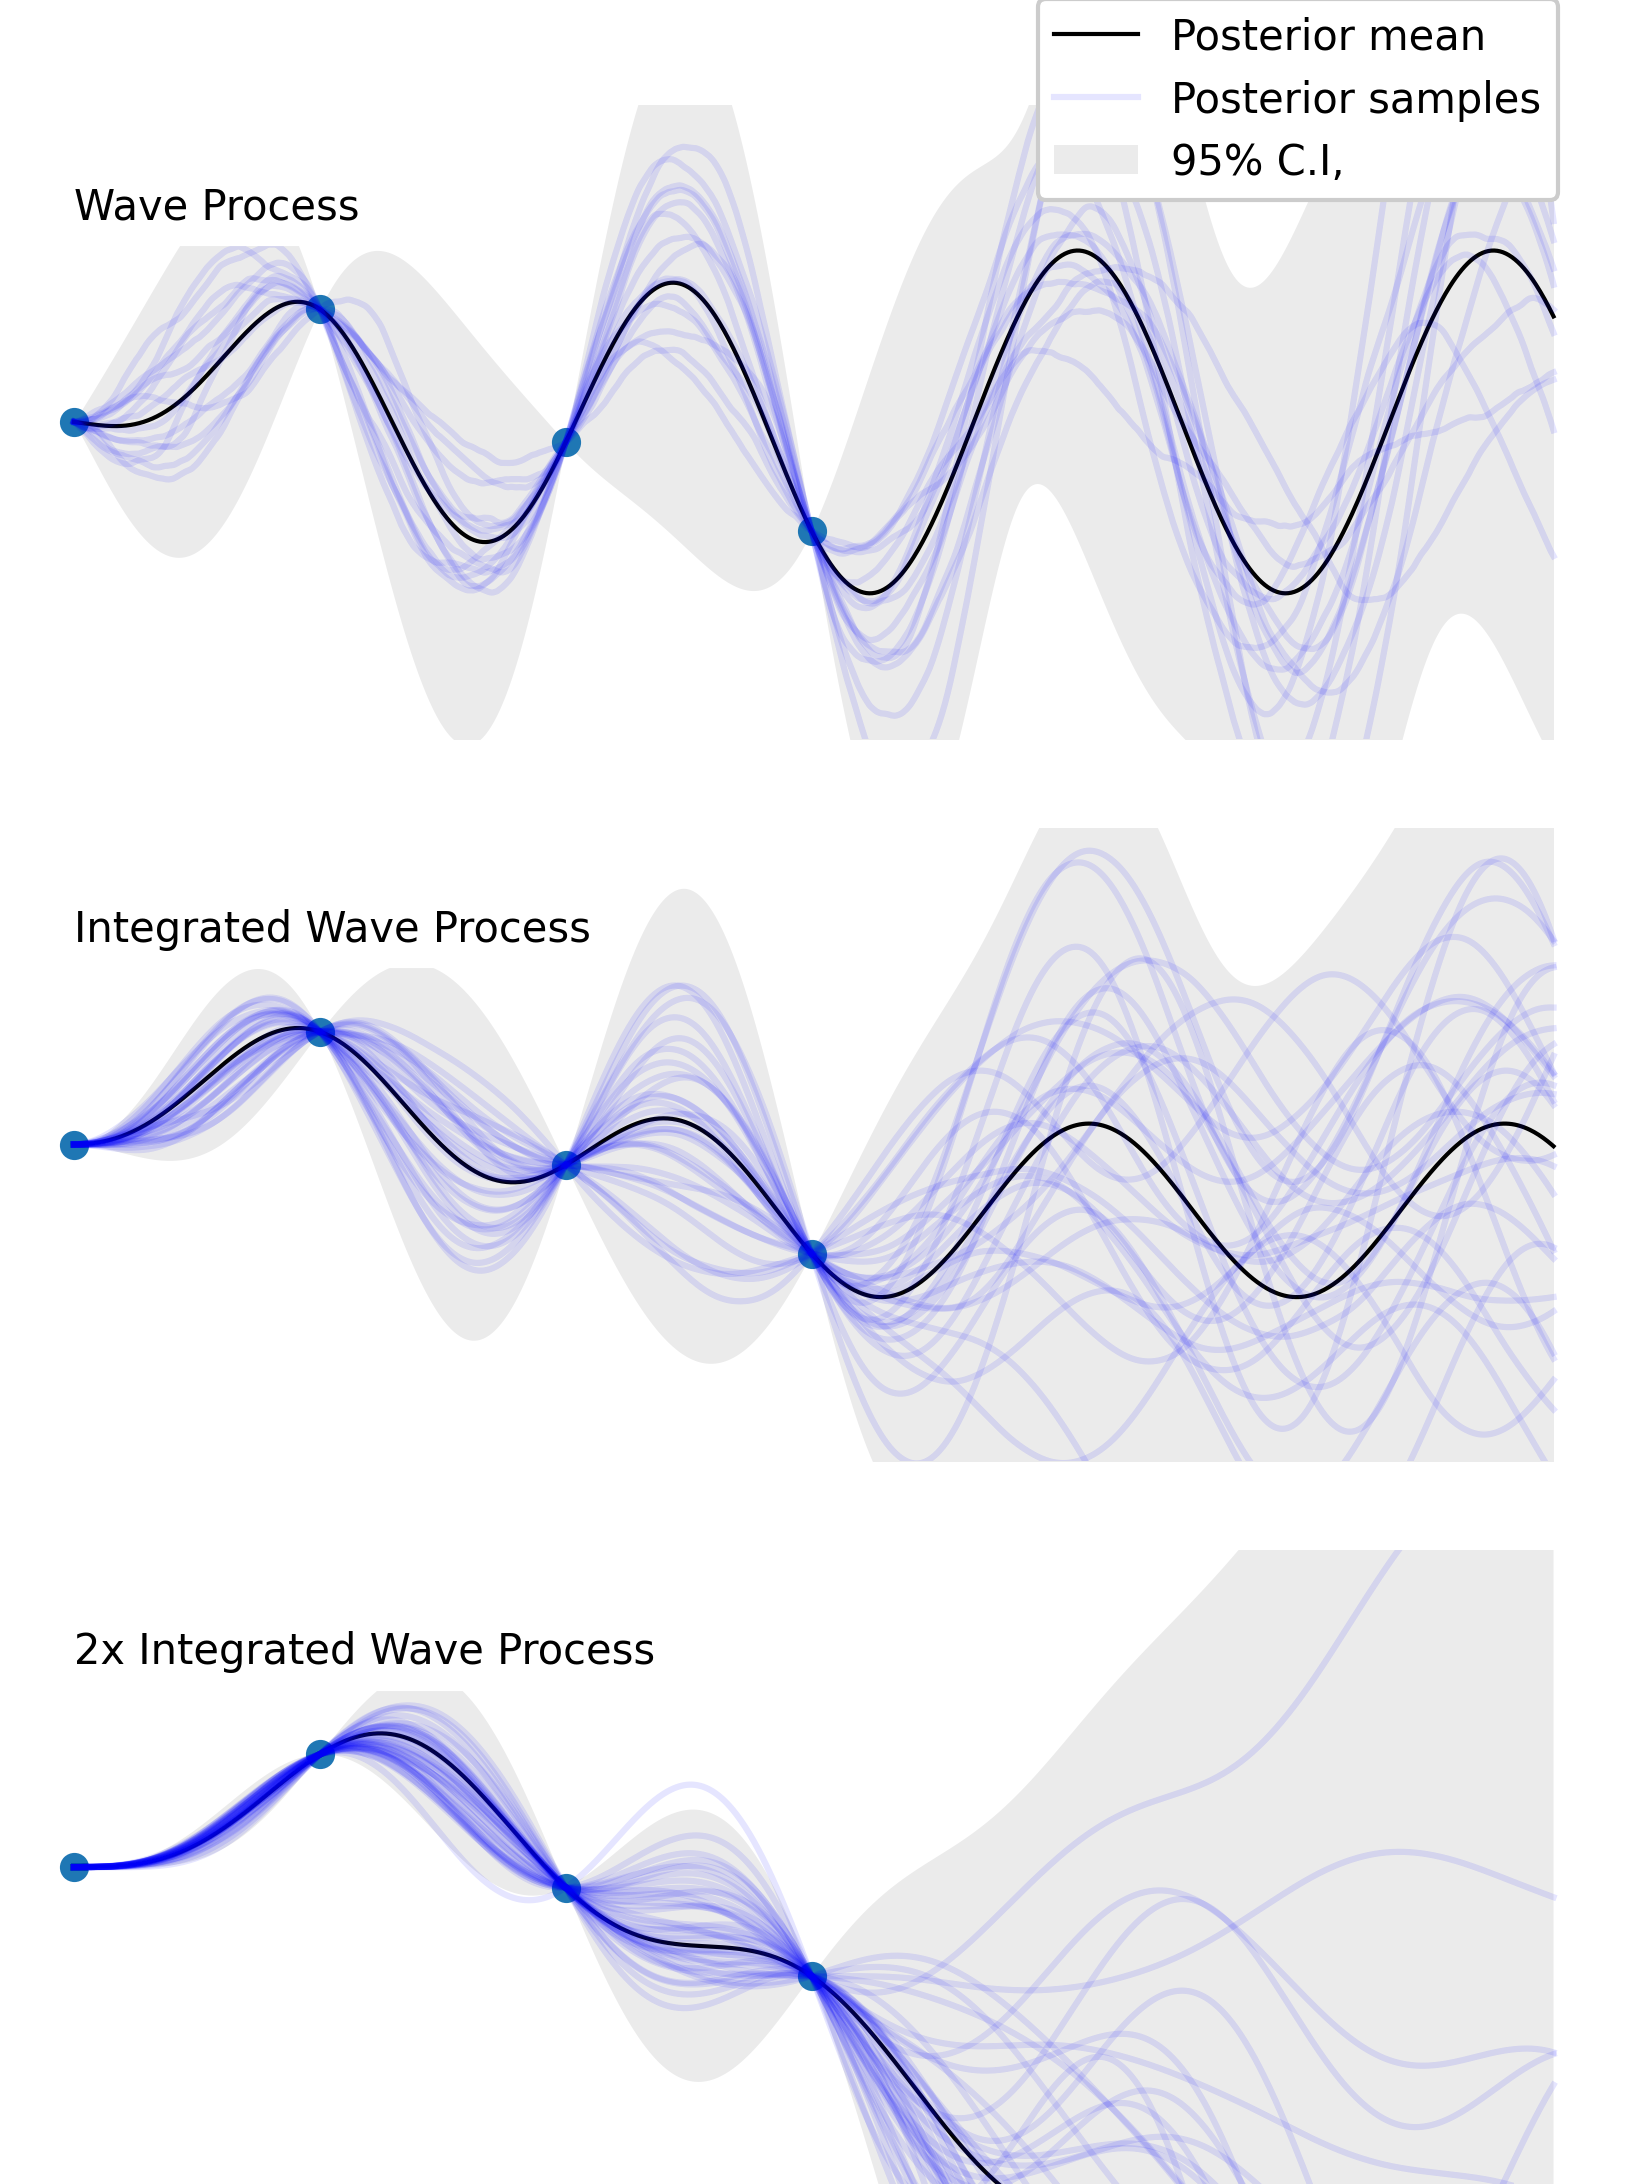
\includegraphics[width=\columnwidth]{../images/conditioned_waves.png}
    \captionof{figure}{Draws from the Integrated Wave Process, Conditioned on the same four points that were also used in chapter \ref{sec:prior}.}
\end{center}
}
\noindent
One is tempted to define a Heat process analogously by placing the Laplacian in the bottom right corner of the dynamics matrix $F$ (which is the correct way of doing it), but it turns out that this reduces to an instance of the Ornstein-Uhlenbeck process with a specific setting of the rate-parameter. We will still refer to it as the Heat process / prior, which captures the spatial diffusion encoded in $L$.

\subsection*{Experiments}
We empirically investigate the efficiency of the probabilistic solver when using the integrated Wiener process, the integrated Wave process, and the integrated heat process as priors for the nonlinear heat and wave equations (eq. \ref{eq:nonlinear_heat} \& \ref{eq:nonlinear_wave}).
As the nonlinearities become larger and we move away from the linear dynamics, the prior will not as related and we should expect a decrease in efficiency.  We run both problems for $\alpha\in\{0, 10^{-3}, 1\}$.
\\
For eq. \ref{eq:nonlinear_heat} we will use the Heat processes, and for eq. \ref{eq:nonlinear_wave}, we will use integrated Wave processes as our prior. We will compare against repeatedly integrated Wiener processes as priors.
\\\\
The problems will be solved on the 2D surface of the sphere, approximated by a 12-vertex icosphere. The vector fields are integrated from $t_0=0$ to $t_{\mathbb{T}}=10$.  We will grade the PN solutions by the root-mean-square-error at all computed timesteps against a high-accuracy reference solution implemented in \texttt{diffrax} \cite{diffrax}, using the Kvaerno5/4 method \cite{kvaerno}, suitable for stiff problems like the heat and wave equation. The reference solution has both relative and absolute tolerances of $10^{-8}$, which then also serves as a lower bound for the error of the PN solution.
\\ The PN solution will be computed for varying amount of timesteps and for different choices of $q$ in the prior process. We will then plot the work/precision diagrams for the different choices of $q$ and $a$.
\subsection*{Results}
See figures \ref{fig:heat big} through \ref{fig:wave big} for all work/precision diagrams. In the figures, the integrated Wiener process is depicted in green, the integrated Wave process in blue, and the integrated heat process in red. The x-axis shows the number of timesteps in the discretized prior ($|\mathbb{T}|$), and the y-axis shows the root-mean-square-error. As the number of steps increase, the error generally decreases. For increasing $q$, the error drops faster.
\\ The integrated Wiener processes are generally being outperformed, however less decisively so for significant nonlinearities ($a = 1$). For $a=0$ the expected exact solution of the priors is observed, even for $10$ timesteps, massively outperforming the integrated Wiener process (but this was not a fair competition).
\\ The result confirm that an appropriate prior process gives the solver an inductive bias that helps solve the ODEs more exactly and efficiently.
\begin{center}
    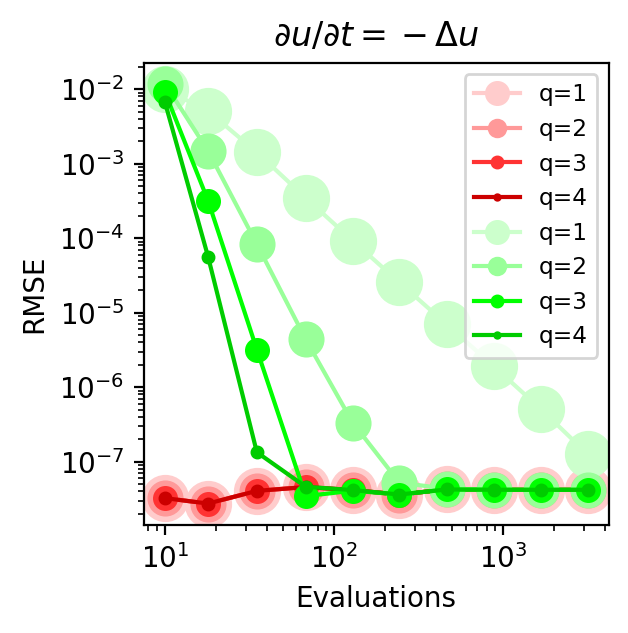
\includegraphics[width=\columnwidth]{../images/solver_heat.png}
    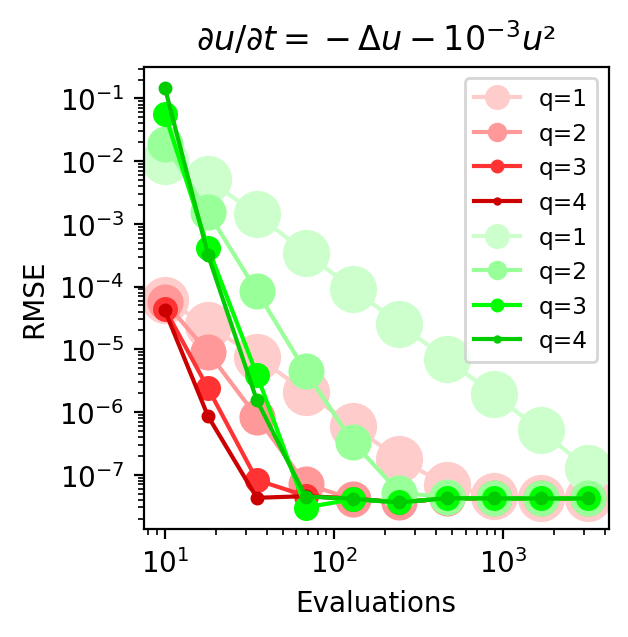
\includegraphics[width=\columnwidth]{../images/solver_heat and medium square.png}
    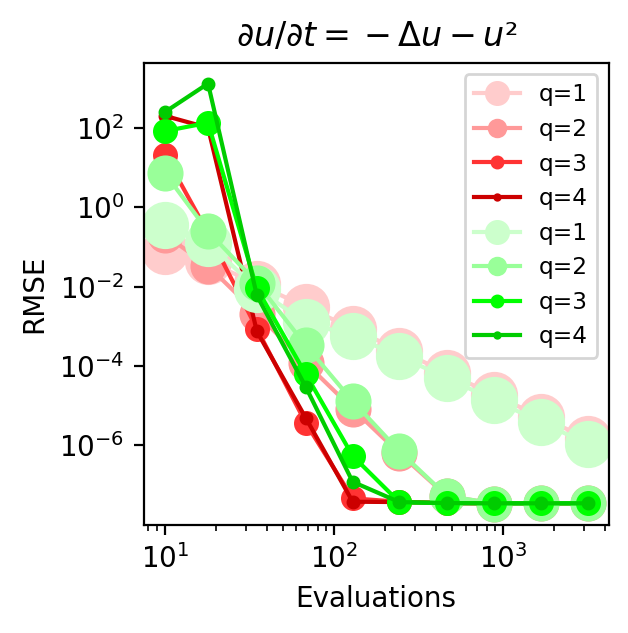
\includegraphics[width=\columnwidth]{../images/solver_heat and big square.png}
    \captionof{figure}{}
    \label{fig:heat big}
\end{center}
\begin{center}
    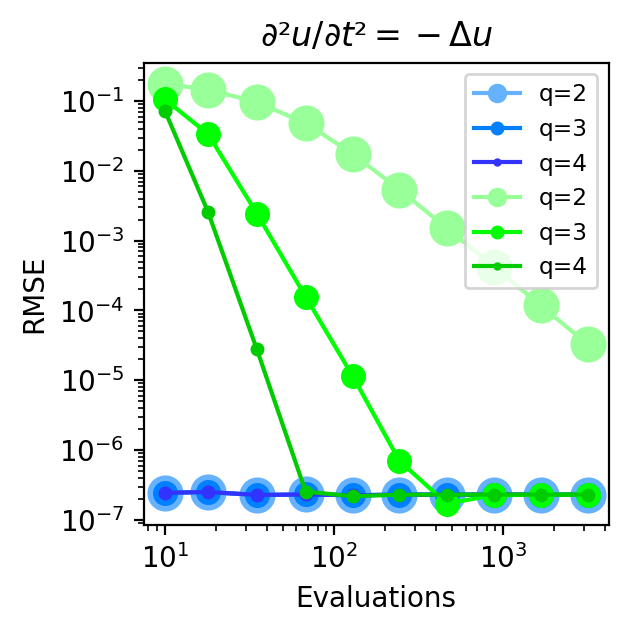
\includegraphics[width=\columnwidth]{../images/solver_wave.png}
    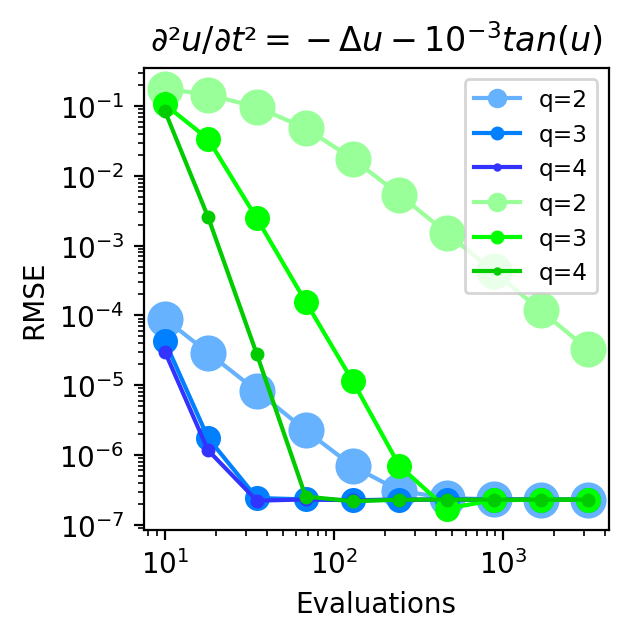
\includegraphics[width=\columnwidth]{../images/solver_wave and medium tan.png}
    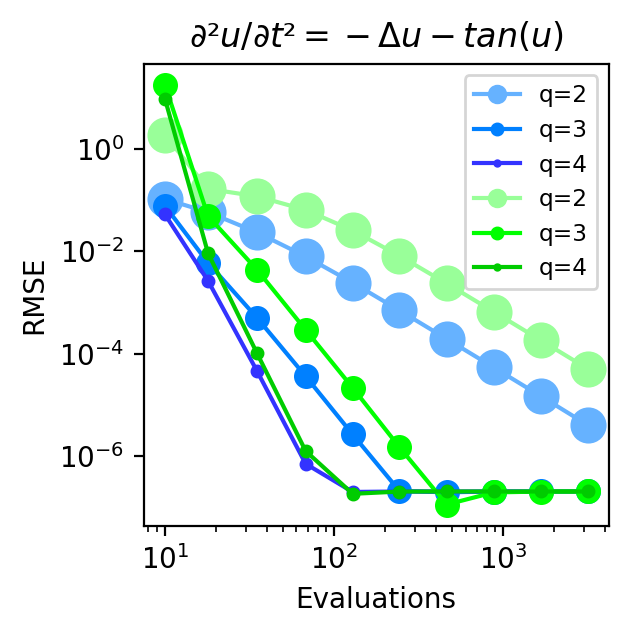
\includegraphics[width=\columnwidth]{../images/solver_wave and big tan.png}
    \captionof{figure}{}
    \label{fig:wave big}
\end{center}


\ifdefined\COMPILINGFROMMAIN
\else    
    \end{document}
\fi